\documentclass[english, a4paper,12pt]{article}
\usepackage{blindtext} % Lorem ipsum
% Packages
\usepackage[a4paper,includeheadfoot,margin=2cm]{geometry} % Layout ,showframe
\usepackage{caption}
\usepackage[hidelinks]{hyperref} %links within the document and for clickable URLs
\usepackage{graphicx}
\usepackage{amsmath} % equations

\usepackage[backend=bibtex,style=ieee]{biblatex} % or verbose-trad2
\bibliography{source.bib} % add sources to source.bib file
% https://www.latex-tutorial.com/tutorials/bibtex/

\usepackage{titling} % So you can use theauthor

\usepackage[hybrid]{markdown} % Used to convert markdown
% pdflatex --shell-escape
%https://www.overleaf.com/learn/latex/Articles/How_to_write_in_Markdown_on_Overleaf

%Bild
\graphicspath{{img/}}
\usepackage{float} % Allows putting an [H] (place HERE & not where LaTeX wants to put)

\usepackage{fancyhdr} % Header & Footer

% Für Deutsch
%\usepackage[utf8]{inputenc}
%\usepackage[ngerman]{babel} --- für deutsh

\usepackage{siunitx} % Required for alignment
\sisetup{
	round-mode          = places, % Rounds numbers
	round-precision     = 2, % to 2 places
}
\usepackage{booktabs} % For prettier tables

% TODO: better Title page
% Document information
\title{ZHAWo - Platform Independent Timetable App}
\author{Bachmann Dominik, Visser Julian}

% Header & Footer
\pagestyle{fancy}
\fancyhf{}
\lhead{PA - 2018}
\chead{ZHAWo}
\rhead{\theauthor}
\lfoot{}
\cfoot{\thepage}
\rfoot{}

\begin{document}

	% !TEX root = pa_doc.tex

%----------------------------------------------------------------------------------------
%	TITLE PAGE
%----------------------------------------------------------------------------------------
\begin{titlepage} % Suppresses displaying the page number on the title page and the subsequent page counts as page 1
	\newcommand{\HRule}{\rule{\linewidth}{0.5mm}} % Defines a new command for horizontal lines, change thickness here

	\center % Centre everything on the page

	%------------------------------------------------
	%	Headings
	%------------------------------------------------

	
\includegraphics[width=0.3\textwidth, left]{./assets/zhawLogo.jpeg}\\[1cm]

	\textsc{\Large Projekt Arbeit}\\[0.5cm] % Major heading such as course name

	\textsc{\large HS 2018}\\[0.5cm] % Minor heading such as course title

	%------------------------------------------------
	%	Title
	%------------------------------------------------

	\HRule\\[0.5cm]

	%------------------------------------------------
	%	Logo
	%------------------------------------------------

	
\includegraphics[width=0.4\textwidth]{./assets/zhawoLogo.png}\\[0.5cm]

	\textsc{\large \textbf{ZHAWo} \\[0.2cm]
									--- \\[0.3cm]}
	% Title of your document
	\textsc{\large Platform Independent Timetable App}\\[0.5cm]


	\HRule\\[1cm]

	%------------------------------------------------
	%	Author(s)
	%------------------------------------------------

	\begin{minipage}{0.4\textwidth}
		\begin{flushleft}
			\large
			\textit{Authors}\\
			Bachmann Dominik \\
			Visser Julian % Your name
		\end{flushleft}
	\end{minipage}
	~
	\begin{minipage}{0.4\textwidth}
		\begin{flushright}
			\large
			\textit{Supervisor}\\
			Meier Andreas % Supervisor's name
		\end{flushright}
	\end{minipage}

	%----------------------------------------------------------------------------------------

	%------------------------------------------------
	%	Date
	%------------------------------------------------
	\vfill
	{\large\today} % Date, change the \today to a set date if you want to be precise

\end{titlepage}


	\pagenumbering{gobble}


	%Index
	\newpage
	\pagenumbering{roman}
	\tableofcontents
	\newpage
	%Abstract
	% !TEX root = pa_doc.tex
\begin{abstract}
\begin{markdown}

\noindent Where is my next lecture? Is there a free room for me to study in? What is the Lunch Menu today?

\noindent These are just a few of the many questions Students have to deal with daily and getting an anwser to these questions isn't always that easy.

\noindent Our vision for zhawo is to solve this. All the information regarding your life a the ZHAW in one place.

\noindent We want to provide our Users a fast, Reliable and Engaging experience across all Platforms. That is why we have chosen to develop zhawo as a Progressive Web App. Progressive Web Apps are web apps that behave like native apps. That means the application can be accessed by any device that has a browser, whilst still gives the user the look and feel of a native app.
\end{markdown}
\end{abstract}


	% Main body of your document
	\newpage
	\pagenumbering{arabic}

	%\markdownInput{example.md}

	% !TEX root = pa_doc.tex
\begin{markdown}

# Introduction

Students of the Zürcher Hochschule für Angewandte Wissenschaften (ZHAW) vist mutliple websites daily in order to get the information they need.

\begin{itemize}
  \item \textbf{School Scedule}: http://stundenplan.zhaw.ch/
  \item \textbf{Menu plan}: http://technikum.sv-restaurant.ch/de/menuplan/: Menu plan
  \item \textbf{School events}: https://www.vszhaw.ch/events/
  \item \textbf{Find free Rooms}: Go from room to room
\end{itemize}

% TODO change this sentence below -> less complicated
% bitz en ahgriff nid?

However, apart from the official Android application \cite{DUMMY}, they are either not well suited for use on mobile devices in the case of the official schedule site \cite{DUMMY} or feel outdated.

% TODO write something about issue of maintaining code for both Android and Iphone


By using progressive web application (PWA) technologies \cite{OurReadme} we were able to build a Cross-Platform application.
We want to provide our Users a fast, Reliable and Engaging experience across all Platforms. That is why we have chosen to develop zhawo as a Progressive Web App. Progressive Web Apps are web apps that behave like native apps. That means the application can be accessed by any device that has a browser, whilst still gives the user the look and feel of a native app.

<<<<<<< HEAD
## Goals & Primary Functions
=======


## Goals + Primary Functions
>>>>>>> b0997382d9c860904ff601469f3ebc1d9526fd72
%TODO how to make &

\begin{itemize}
  \item \textbf{Timetable}: students often need to quickly check what courses they have next and where they need to go. The availability of this feature is very important and has been noted as being an issue with the "official" timetable app. Using intelligent caching and a modern user interface, we aim to improve this aspect.
  \item \textbf{Room search}: when we first started there was an application, that allowed students to search for free rooms all over their campus. This was very useful as study programmes at the ZHAW put a huge focus on group projects, but with limited quiet public working spaces, finding a free room was often vital. The app that only ever existed for Android devices has since completely disappeared.
  \item \textbf{Menu plans}: There are menu plans on the official provider of the mensa food's website. However, this site is rather unknown and we plan to include an easy way to check today's and upcoming menus and prices.
  \item \textbf{Student events}: We plan to work with vszhaw to bring more attention to student parties and events, by integrating their event feed into zhawo.
\end{itemize}

\end{markdown}

  \newpage
  
  % !TEX root = pa_doc.tex
\begin{markdown}
# Technologies

*add an intro*

## PWA
\say{Progressive Web Apps (PWA) are experiences that combine the best of the web and the best of apps.}\cite{WhatIsPWA}

Google and other companies have developed a new, modern web application standard. PWAs implement said standard and receive additional permission as a rewarded for doing so. This allows PWA to behave and feel like native apps. They live can on the user's home screen, offer a full screen experience, access device hardware (camera, GPS, etc) and can even re-engage users with push notifications\cite{PWA}.  When launched from the user’s home screen a Progressive Web App can load instantly, regardless of the network state. This is done by with the help of service workers.

### Service Workers
A service worker is like a client-side proxy and that allows control of the cache. You can improve the loading speed of your page by pre-caching key resources. Using cache also eliminates the dependence on the network, ensuring a reliable offline experience for your users.\cite{ServiceWorker}

## React
React\cite{React} was originaly developed by Facebook and is one of the most popular UI librarys. It allows you to create reusable Compents using JSX, a syntax extension to JavaScript.
The idea behind React is to design simple views for each state of the application. Doing so allows it to only update and render components that need to be changed, thereby improving performance immensely.

### Flux
Flux\cite{OurReadme} is a application pattern developed by Facebook. It's goal is to insure a a unidirectional data flow in React apps. The use of this practice enhances the quality and performance of the code by improving the data consistency. It is the optimal architecture for the use of React.

\begin{figure}[H]
  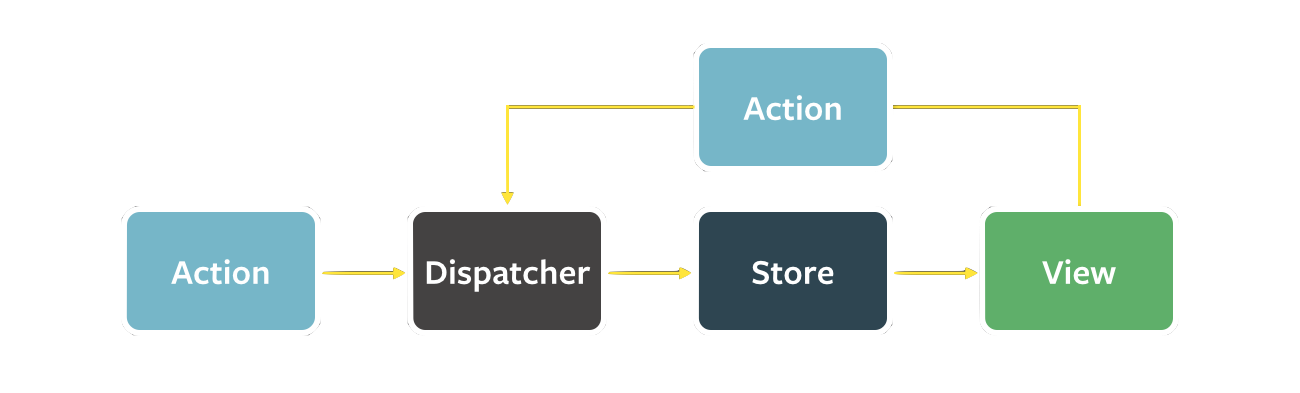
\includegraphics[width=10cm, center]{./assets/flux.png}
  \caption{Flux Model{\cite{FluxModel}}}
\end{figure}



% TODO: bild ref https://facebook.github.io/flux/img/flux-simple-f8-diagram-with-client-action-1300w.png

In Flux, the dispatcher is a singleton that directs the flow of data to ensure that updates do not cascade, which would lead to unpredictable behaviour. When a user interacts with a React view, the view sends an action through the dispatcher, which notifies the stores that hold the application’s data. When the stores change state, the view gets notified and changes accordingly.

## NodeJS
Node.js is a JavaScript runtime environment, designed to build scalable network applications\cite{Node}.
*öpis vo da https://nodejs.org/en/about/* blocking and so on
### Express
Express\cite{Express} is a minimal and flexible web application framework for Node.js. It provides HTTP utility methods and allows you to create a robust API.
With just a few lines of Code you have a WebServer up and running.

% TODO: failt
% \begin{lstlisting}
% const express = require('express');
% const app = express();

% app.get('/', (req, res) => {
%     res.send('An alligator approaches!');
% });

% app.listen(3000, () => console.log('Gator app listening on port 3000!'));
% \end{lstlisting}

\end{markdown}

  \newpage

  % !TEX root = pa_doc.tex
\begin{markdown}

# Implementation

Explain Architecture, Flux pattern (unidirectional flow), maybe some diagrams
    
\end{markdown}
  \newpage

  % !TEX root = pa_doc.tex
\begin{markdown}

# Discussion

Over the past Semester we built fast and reliable prototype of ZHAWo as a PWA. Users can login using there ZHAW username, view thier timetable and look for free Room. They can also access menu plans of the different campus mensas or read the vszhaw blog using our app.

Our initial goals were met and the initial feedback has been positive. Nevertheless, our application still needs further optimisation before it can be used in a productive environment. There are also additional features that we would like to add, that will further improve the experience of our users.

TODO: pwas and javascript promising for 

\end{markdown}

  \newpage

	\section{Appendix}

	\listoffigures
	\listoftables
	%\renewcommand\refname{Literaturverzeichnis}% rename --- für deutsh
	\printbibliography  % Uses source.bib to make ref table

\end{document}
